
From the given information,
\begin{align}
\vec{m}=\myvec{1\\\frac{1}{\sqrt{3}}},c=-2
\end{align}
The normal vector of the line is
\begin{align}
\vec{n}=\myvec{\frac{-1}{\sqrt{3}}\\1}
\end{align}
Equation of the line in terms of the normal vector is then obtained as
\begin{align}
\vec{n}^{T}\vec{x}&=c
//
\implies \myvec{-1 & \sqrt{3}}\vec{x}=-2\sqrt{3}\label{5/3/fe}
\end{align}
See Fig.         \ref{5/3/fig:Line} 
\begin{figure}[ht!]
       \centering
        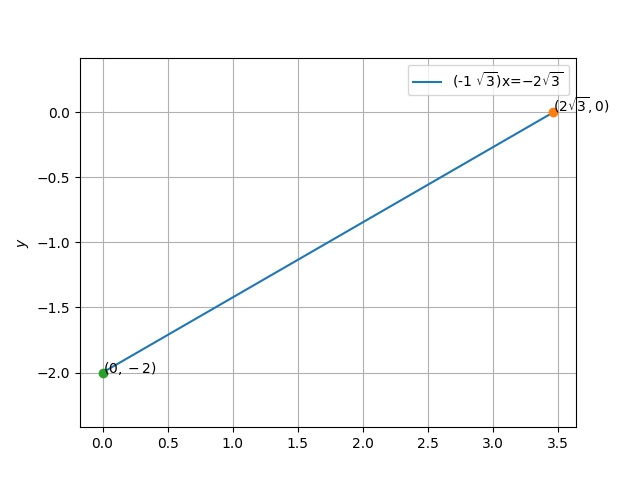
\includegraphics[width =\columnwidth]{fig2.1.png}
        \caption{Plot obtained from python code.We get the required equation.$\myvec{-1 & \sqrt{3}}\vec{x}=-2\sqrt{3}$}
        \label{5/3/fig:Line}
\end{figure}


